\chapter{Глава 4}\label{ch:ch4}

\section{Устройство относительного измерения момента}\label{sec:ch4/sect1}


В филиале АО «Корпорация «Комета» – «НПЦ ОЭКН» создано и и аттестовано устройство относительного измерения остаточного момента (УОИОМ). На рисунке \cref{fig:yoim} представлен общий вид установки.

\begin{figure}[ht]
	\centerfloat{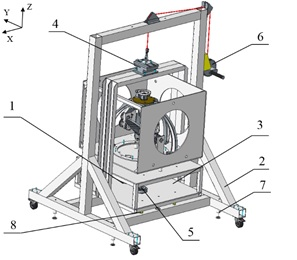
\includegraphics[scale=2]{yoiom}}
	\caption{Устройство относительного измерения остаточного момента}
	\legend{1 – маховик; 2 – платформа; 3 – измерительная платформа с изделиедержателем; 4 – зацеп настраиваемый; 5 – узел привода редукторного OZ; 6 – привод редукторный OZ;
	 7 – волконно-оптический гироскоп; 8 – конус}
	\label{fig:yoim}
\end{figure}

Стенд для измерения остаточного реактивного момента представляет собой конструкцию, обеспечивающую измеряемой аппаратуре одну степень свободы, без сухого трения. В процессе углового перемещения ОМС на основание аппаратуры действует реактивный момент. Частично этот момент компенсируется маховиками, входящими в состав ОМС. Таким образом,
стенд служит для измерения некомпенсированного внутренними средствами аппаратуры реактивного момента. Конструктивно стенд представляет собой 
крутильный маятник. Момент инерции маятника состоит из суммы моментов инерции рамы с кантователем и момента инерции аппаратуры по измеряемой оси. Кантователь входит в узел подвеса и служит для удобства 
смены измеряемой оси аппаратуры путем расположения этой оси строго вертикально по оси чувствительности подвеса. Дифференциальное уравнение колебательного звена крутильного маятника запишем  в виде [13]

\begin{samepage}
	\begin{equation}
		\label{eq:eq_yoimDiff}
		\begin{alignedat}{2}
			J\ddot{\phi}\left(t\right) + 2b\dot{\phi}\left(t\right)+c\phi\left(t\right) = M\left(t\right)
		\end{alignedat}
	\end{equation}
	\begin{align*}
		\text{где}	& \quad J - \textnormal{момент инерции;}\\           
		& \quad b - \textnormal{обобщённое вязкое трение;}        \\
		& \quad c -  \textnormal{угловая жесткость подвеса;} \\
		& \quad M(t) - \textnormal{внешний момент;}         \\
		& \quad \phi(t) -\textnormal{угол порота узла подвеса} \\
	\end{align*}
\end{samepage}

Запишем уравнение~\cref{eq:eq_yoimDiff} иначе:ъ

\begin{samepage}
	\begin{equation}
		\label{eq:eq_yoimDiff2}
		\begin{alignedat}{2}
			\phi\left(t\right)+2\xi\phi\left(t\right)+\omega_{0}^2\phi\left(t\right) = M\left(t\right)/J
		\end{alignedat}
\end{equation}
\begin{align*}
	\text{где}	& \quad \omega_0 - \textnormal{собственная частота колебательного звена;}\\           
	& \quad \xi - \textnormal{декремент затухания;}        \\
\end{align*}
\end{samepage}


На рисунке~\cref{fig:amplitude-freq-char} представлены логарифмические амплитудная и фазовая характеристики колебательного звена. Характеристики построены относительно резонансной (собственной) частоты.

\begin{figure}[ht]
	\centerfloat{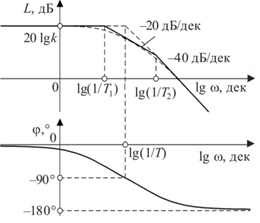
\includegraphics[scale=2]{amplitude-freq-char}}
	\caption{ЛАЧХ колебательного звена}
	\label{fig:amplitude-freq-char}
\end{figure}


Как видно из рисунка, колебательное звено не искажает входного сигнала ни по амплитуде вплоть до области, близкой к собственной частоте колебаний. В области частот выше собственной выходной сигнал подавляется с темпом \SI{-40}{\text{дБ/декада}}, а фаза выходного сигнала сдвигается на $\pi$ по отношению к фазе входного входного сигнала[14]. Если выходной сигнал состоит из нескольких гармоник, то в этой области частот высокочастотные гармоники будут ослабляться по мере удаления от частоты резонанса. Таким образом, с точки зрения информативности измерений наиболее рационально работать в дорезонансной области частот, где угловые перемещения узла подвеса наилучшим образом соответствуют действию моментов на узел подвеса.

Зададим внешний момент в виде функции, представленной на рисунке~\cref{fig:external_moment}, и разложим её в ряд Фурье [15]



\begin{samepage}
	\begin{equation}
		\label{eq:furie}
		\begin{alignedat}{2}
		M(t) = \frac{4 \alpha}{\pi} \cos\left(\frac{\pi}{4}\right) \sin\left(\omega t\right) + \\
				1/3 \cos\left(\frac{3\pi}{4} \right) \sin\left(3\omega t \right) + \\
				1/5 \cos \left(\frac{5 \pi}{4} \right) \sin \left(5 \omega t\right) + \\
				1/7 \cos \left(\frac{7 \pi}{4} \right) \sin \left(7 \omega t \right) + \\
				1/9 \cos \left(\frac{9 \pi}{4} \right) \sin \left(9 \omega t \right)+ ...
		\end{alignedat}
	\end{equation}
	\begin{align*}
		\text{где}	& \quad \alpha - \textnormal{собственная частота колебательного звена;}\\           
	\end{align*}
\end{samepage}

На рисунке~\cref{fig:external_moment_furie} приведены упрощенный график остаточного реактивного, возникающего при тестовом воздействии маховика, и результат суммирования первых шести слагаемых ряда Фурье~\cref{eq:furie}. Пропустим шесть первых гармоник ряда Фурье через колебательное звено~\cref{eq:eq_yoimDiff} последовательно и суммируем полученные результаты. 

Для каждой из гармоник угла отклонения рамы стенда можно записать :


\todo{Формулы}


В соответствии с заданием на проектирование аппаратуры - первая гармоника возмущающего момента имеет период $T_1 = \SI{4}{c}$(Время периода вращения оптической системы) и круговую частоту $\omega_{r_1} = \frac{1}/{T_1} = \SI{0,25}{рад/c}$.

На рисунке~\cref{fig:decrement} приведен результат результат моделирования ускорения рамы под действием момента при различных настройках узла подвеса стенда с различными декрементами затухания и $T_1 = \SI{4}{c}$. На рисунке~\cref{fig:decrement} видно, что увеличение декремента затухания больше $\xi = 0,1$ приводит к существенным деформациям





